

\chapter{\eigenTitle}
\label{eigenvalseigenvects}

In a vector space with no structure other than the vector space rules, no vector other than the zero vector  is any  more important than any other.
Once one also has a linear transformation the situation changes dramatically. We begin with a fun example, of a type bound to reappear in your future scientific studies:

\begin{example}[String Theory]

Consider a vibrating string, 
whose displacement at point $x$ at time $t$ is given by a function $y(x,t)$:
\begin{center}
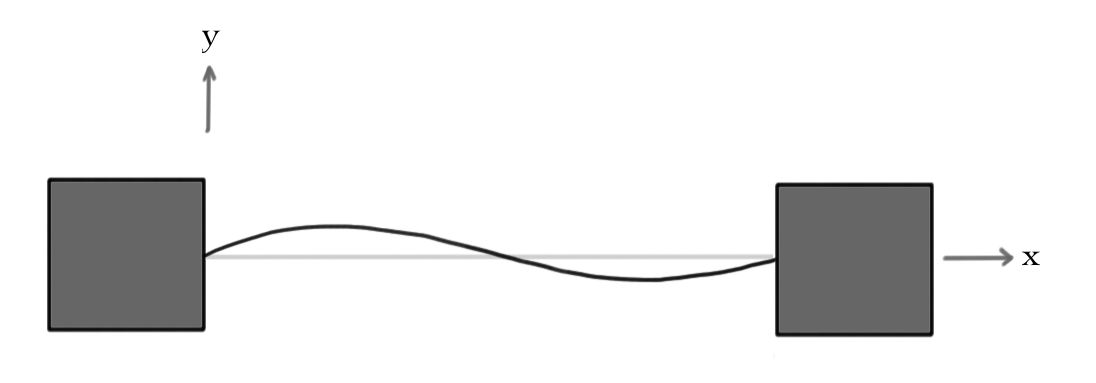
\includegraphics[scale=.3]{string.jpg}
\end{center}
The set of all displacement functions for the string 
can be modeled by 
a vector space 
\[V=\left\{ y:\mathbb{R}^2 \to \mathbb{R} \middle| \mbox{\rm all partial derivatives } \frac{\partial^{k+m}y(x,t)}{\partial x^k\partial t^m} \mbox{ exist}\right\}.\] 
%The reason for the condition that the second derivatives exist is 
 The concavity and 
 the acceleration of the string at the point $(x,t)$ are 
 $\frac{\partial^2y}{\partial x^2}(x,t)$ and $\frac{\partial^2y}{\partial t^2}(x,t)$ respectively. 
 Since quantities must exist at each point on the string for the wave equation to make sense, 
 we required that all partial derivatives of $y(x,t)$ exist.
 Note also that the function $y(x,t)=0$~---drawn in grey---is the only special vector in the vector space~$V$. 

%
We now add some extra information.
The string's behavior in time and space can be modeled by a wave equation\index{Wave equation}
\[\frac{\partial^2 y}{\partial t^2}=\frac{\partial^2 y}{\partial x^2}\, ,
\]
which says that the acceleration of a point on the string is equal its concavity at that point. For example, if the string were made of stretched rubber, it would 
prefer to be in a straight line, so this equation makes good intuitive sense. 
Not all of the functions in $V$ are solutions to the wave equation; not all of the functions in the vector space $V$ describe the way a string would really vibrate.  The ways a string  would really  vibrate are (at least approximately) solutions to the wave equation above, which can rewritten as a linear function
\[Wy=0\]
where
\[
W=\left(-\frac{\partial^2 }{\partial t^2}+\frac{\partial^2 }{\partial x^2}\right):V\rightarrow V\, .
\]
Some examples of solutions are 
\[
y_1(x,t)=\sin (t) \sin (x)\, \quad
y_2(x,t)=3\sin (2t) \sin (2x)\, \]
and
\[
y_3(x,t)=\sin (t) \sin (x)+3\sin (2t) \sin (2x)\, .
\]
Since $Wy=0$ is a homogeneous linear equation, linear combinations of solutions are solutions; in other words the kernel $\ker(w)$ is a vector space.
Given the linear function $W$, some vectors are now more special than others.

We can use musical intuition to do more! If the ends of the string were held fixed, we suspect that it would prefer to vibrate at certain frequencies corresponding to musical notes.
This is modeled by looking at solutions of the form
\[
y(x,t)=\sin(\omega t) v(x)\, .
\]
Here the periodic sine function accounts for the string's vibratory motion, while the function $v(x)$ gives the shape of the string at any fixed instant of time. Observe that
\[
W\big(\sin(\omega t) v(x)\big)=\sin(\omega t)\big(\frac{d^2f}{dx^2}+\omega^2 f\big)\, .
\]
This suggests we introduce a new vector space \[U=\left\{v:{\mathbb R}\to {\mathbb R}\, \middle| \, \mbox{\rm all derivatives } \frac{d^kf}{d x^k }\text{~exist~} \right\}\, ,
\]
as well as a new linear function
\[
L:=\frac{d^2}{dx^2}: U\longrightarrow U\, .
\]
The number $\omega$ is called an angular frequency in many contexts, lets call its square $\lambda:=-\omega^2$ to match notations we will use later (notice that for this particular problem $\lambda$ must then  be negative).
Then, because we want $W(y)=0$, which implies $d^2 f/dx^2=\omega^2 f$, it follows that the vector $v(x)\in U$ determining the vibrating string's shape obeys
\[
L(v)=\lambda v\, .
\]
This is perhaps one of the most important equations in all of linear algebra! It is the eigenvalue-eigenvector equation. In this problem we have to solve it both for $\lambda$, to determine which frequencies (or musical notes) our string likes to sing, and the vector $v$ determining the string's shape. The vector $v$ is called an eigenvector and $\lambda$ its corresponding eigenvalue.
%We can incorporate a realistic complication into our model of the string: 
%an additional force may be pulling the string toward the rest position with a Hooke's law type force. In this case there are two causes for acceleration of a point on the string: the concavity and  Hooke's force.  
%In this case the acceleration of the string at each point will be the sum of the acceleration due to its concavity and the acceleration due to gravity $g$;
%\[\frac{\partial^2 y}{\partial t^2}=\frac{\partial^2 y}{\partial x^2}+ky\, ,
%\]
%or, written as a linear equation 
%\[Ly=ky.\]
%The solution set this of  equation will be different for every different value of the spring constant $k$. 
The solution sets for each $\lambda$ are called $V_\lambda$. For any $\lambda$ the set $V_k$ is a vector space since elements of this set are solutions to the homogeneous equation $(L-\lambda)v=0.$ 



\end{example}

We began this chapter by stating ``In a vector space, with no other structure, no vector is more important than any other." Our aim is  to show you that when a linear operator $L$ acts on a vector space, vectors that   solve the equation    $L(v)=\lambda v$ play a central role.

% with the largest value of k are more important than those for smaller values of $k$. 
%You might ask ``more important in what sense?" 
%In the sense that the function $L$ can be built out of the various values of $k$ and the vectors in $V_k$ and the biggest part of that construction is the part with the biggest values of $k$. In particular for some vectors $v_k\in V_k$
%\[L=\sum_{k} k \, v_k \,v_k^t.\]
%We are aware that we have made the startling suggestion that a derivative operator is a linear combination of products of vectors, and we hope that you are intrigued. Lets now return to the simpler case of linear functions which are matrices to develop this idea.




%Before discussing eigenvalues and eigenvectors, we need to understand very well  the relationship between linear transformations and matrices. Let us review the key ideas.
%Consider, as an example the plane ${\mathbb R}^2$
%\begin{center}
%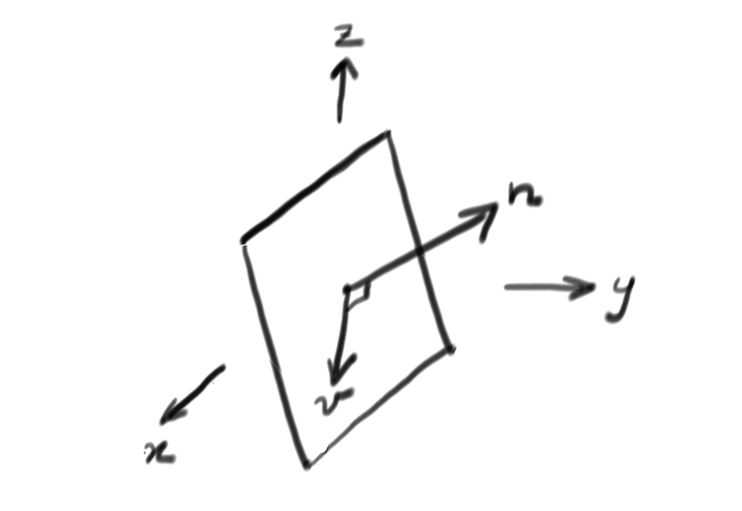
\includegraphics[scale=.3]{\eigenPath/plane.jpg}
%\end{center}
%The  vector $v$ can be described in many ways. 
%Two possibilities are the ordered basis $E=(e_1,e_2)$ 
%and the ordered basis
%$F=(f_1,f_2)$; 
%the vector $v$ is described by the ordered pair $(x,y)^T=(2,2)^T$ in the ordered basis $E$ and by the ordered pair $(s,t)^T=(2,1)^T$ in the ordered basis $F$.  
%This can be confusing! The idea to keep firm in your mind is that the vector space and its elements---vectors---are what really ``exist''. 
%The pairs of numbers are really just different shorthand notations for the same vector. 
%\hyperlink{Basis notation}{Previously} we denoted the correspondence between pairs of numbers and vectors by labeling the pairs of numbers with the basis in which to interpret the numbers;
%\[
%v= \colvec{ 2\\2 }_E :=2e_1+2e_2, ~v= \colvec{2\\1}_F := 2f_1+1f_2\, .
%\]
%
%There is an intuitive reason for the fact that there are many ways to describe the same vector;
%typically, you will use vectors to describe configurations of the real world systems, but the coordinate system you use is your choice. 
%Things like coordinate axes and ``components of a vector'' $(x,y)$ are just mathematical tools used to label vectors.
%
%To generalize this discussion, let $V$ and $W$ be vector spaces, with ordered bases $E=(e_1, \ldots, e_n)$ and 
%$F=(f_1, \ldots, f_m)$ respectively.  
%Since these are bases, there exist constants $v^i$ and $w^j$ such that any vectors $v\in V$ and $w\in W$ can be written as:
%\begin{eqnarray*}
%v & = & v^1e_1 \ + v^2e_2 \ + \cdots + v^ne_n \\
%w & = & w^1f_1 + w^2f_2 + \cdots + w^mf_m \\
%\end{eqnarray*}
%We call the coefficients $v^1, \ldots, v^n$ the \emph{components}\index{Components of a vector} of $v$ in the ordered basis\footnote{To avoid confusion, it helps to note that components of a vector are labeled by a superscript, while basis vectors are labeled by subscripts. This is part of Einstein's notation convention.} $(e_1, \ldots, e_n)$. It is often convenient to arrange the components $v^i$ in a column vector and the basis vectors in a row vector by writing
%\[
%v=\rowvec{e_1 & e_2 & \cdots & e_n}\colvec{v^1 \\ v^2 \\ \vdots \\  v^n}\, .
%\]
%\videoscriptlink{eigenvectors_and_eigenvalues_matrix.mp4}{Worked Example}{scripts_eigenvalseigenvects_matrix}
%
%For what follows it is often convenient follow this order and put the scalar coefficients to the right of basis vectors as in 
%\[v  =  e_1v^1 \ + e_2v^2 \ + \cdots + e_nv^n .\] 
%
%
%
%\begin{example}
%Consider the ordered basis $B=(1-t, 1+t )$ for the vector space of polynomials of order 1 or lower $P_1(t)$.  The vector $v=2t$ has components $v^1=-1, v^2=1$ in the ordered basis $B$ because 
%\[v=(1-t)(-1) + (1+t)1=\rowvec{1-t & 1+t}\colvec{-1 \\[2mm] 1}\, .\]
%\end{example}
%
%When describing general cases the adroit reader will also enjoy the compact Einstein summation notation $v=e_iv^i$.
%
%%We may consider these components as vectors in $\Re^n$ and $\Re^m$:
%%\[
%%\colvec{v^1\\ \vdots \\ v^n}\in \Re^n, \qquad 
%%\colvec{w^1\\ \vdots \\ w^m}\in \Re^m.
%%\]


\section{Invariant Directions}

Have a look at the linear transformation $L$ depicted below:
\begin{center}
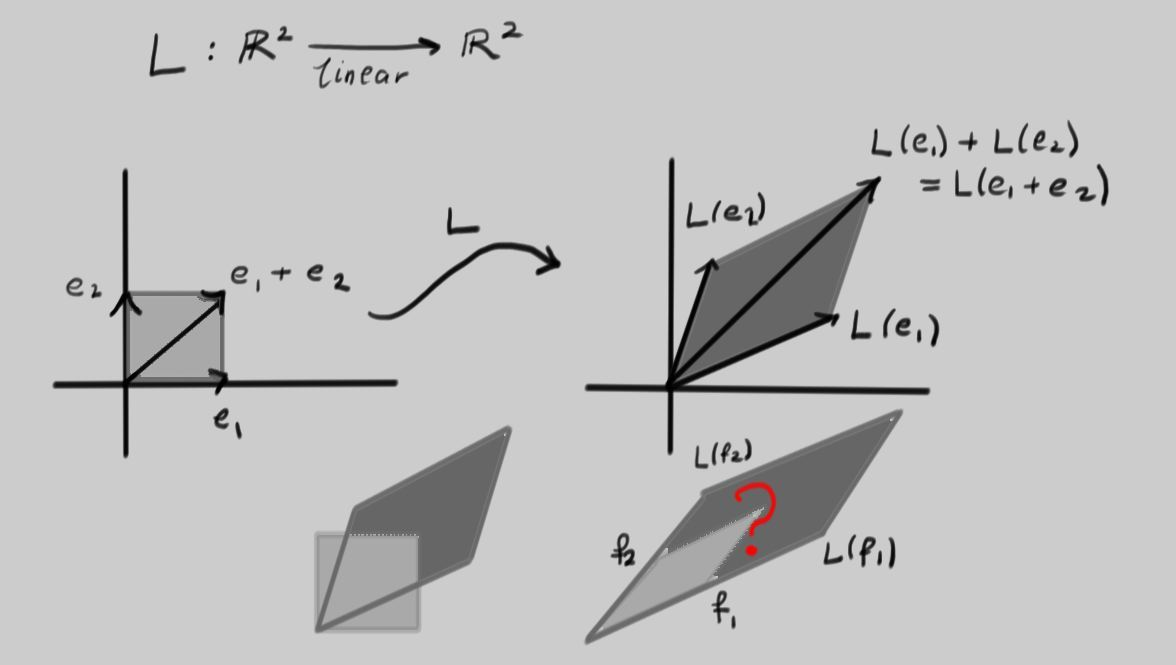
\includegraphics[scale=.3]{\eigenPath/invariant.jpg}
\end{center}
It was picked at random by choosing a pair of vectors $L(e_1)$ and $L(e_2)$ as the outputs of $L$ acting on the canonical basis vectors.
Notice how the unit square with a corner at the origin is mapped to a parallelogram.  The second line of the picture 
shows these superimposed on one another. Now look at the second picture on that line. There, two vectors $f_1$ and $f_2$ have been carefully
chosen such that if the inputs into $L$ are in the parallelogram spanned by $f_1$ and $f_2$, the outputs also form a parallelogram with
edges lying along the same two directions. Clearly this is a very special situation that should correspond to  interesting properties of $L$.

Now lets try an explicit example to see if we can achieve the last picture:

\begin{example}
Consider the linear transformation $L$ such that \[L\colvec{1\\0}=\colvec{-4\\-10}\,  \mbox{ and }\, L\colvec{0\\1}=\colvec{3\\7}\, ,\] so that the matrix of $L$ in the standard basis is \[\begin{pmatrix}
-4 & 3 \\
-10 & 7 \\
\end{pmatrix}\, .\]  Recall that a vector is a direction and a magnitude; $L$ applied to $\colvec{1\\0}$ or $\colvec{0\\1}$ changes both the direction and the magnitude of the vectors given to it.

Notice that \[L\colvec{3\\5}=\colvec{-4\cdot 3+3\cdot 5 \\ -10\cdot 3+7\cdot 5}=\colvec{3\\5}\, .\]  Then $L$ fixes the  direction (and actually also the magnitude) of the vector $v_1=\colvec{3\\5}$.  

%In fact also the vector $v_2=\colvec{1\\2}$ has its direction fixed by $M$ because $Lv_2=2v_2$.



%\begin{center}\href{\webworkurl ReadingHomework18/1/}{Reading homework: problem \ref{eigenvalseigenvects}.1}\end{center}
\Reading{EigenvaluesAndEigenvectors}{1}

Now, notice that any vector with the same direction as $v_1$ can be written as $cv_1$ for some constant $c$.  Then $L(cv_1)=cL(v_1)=cv_1$, so $L$ fixes every vector pointing in the same direction as $v_1$.

Also notice that \[L\colvec{1\\2}=\colvec{-4\cdot 1+3\cdot 2 \\ -10\cdot 1+7\cdot 2}=\colvec{2\\4}=2\colvec{1\\2}\, ,\] so $L$ fixes the direction of the vector $v_2=\colvec{1\\2}$ but stretches $v_2$ by a factor of $2$.  Now notice that for any constant $c$, $L(cv_2)=cL(v_2)=2cv_2$.  Then $L$ stretches every vector pointing in the same direction as $v_2$ by a factor of $2$.

\end{example}

In short, given a linear transformation $L$ it is sometimes possible to find a vector $v\neq 0$ and constant $\lambda\neq 0$ such that 
$
Lv=\lambda v.
$
\begin{figure}
\begin{center}
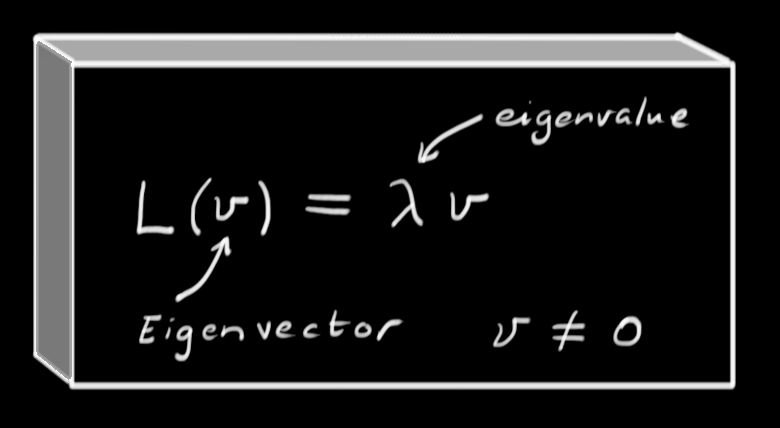
\includegraphics[scale=.4]{\eigenPath/eigeneqn.jpg}
\end{center}
\caption{The eigenvalue--eigenvector equation is probably the most important one in linear algebra.}
\end{figure}
We call the direction of the vector $v$ an \emph{invariant direction}\index{Invariant direction}.  In fact, any vector pointing in the same direction also satisfies this  equation because   $L(cv)=cL(v)=\lambda cv$.  
More generally, any {\itshape non-zero} vector $v$ that solves
\[
L(v)=\lambda v
\]
is called an \emph{eigenvector}\index{Eigenvector} of $L$, and $\lambda$ (which now need not be zero) is an \emph{eigenvalue}\index{Eigenvalue}.  Since the direction is all we really care about here, then any other vector $cv$ (so long as $c\neq 0$) is an equally good choice of eigenvector. Notice that the relation ``\(u\) and \(v\) point in the same direction'' is an equivalence relation.

In our example of the linear transformation $L$ with matrix \[\begin{pmatrix}
-4 & 3 \\
-10 & 7 \\
\end{pmatrix}\, ,\] we have seen that $L$ enjoys the property of having two invariant directions, represented by eigenvectors $v_1$ and $v_2$ with eigenvalues $1$ and $2$, respectively.  

It would be very convenient if we could write any vector $w$ as a linear combination of $v_1$ and $v_2$.  Suppose $w=rv_1+sv_2$ for some constants $r$ and~$s$.  Then
\[
L(w)=L(rv_1+sv_2)=rL(v_1)+sL(v_2)=rv_1+2sv_2.
\]
Now $L$ just multiplies the number $r$ by $1$ and the number $s$ by $2$.  If we could write this as a matrix, it would look like:
\[
\begin{pmatrix}
1 & 0 \\
0 & 2
\end{pmatrix}\colvec{s\\t}
\]
which is much slicker than the usual scenario  \[L\!\begin{pmatrix}
x\\
y
\end{pmatrix}\!=\!\begin{pmatrix}
\!a&b\! \\
\!c&d\!
\end{pmatrix} \! \!\begin{pmatrix}
x \\
y
\end{pmatrix}\!=\!
\begin{pmatrix}
\!ax+by\! \\
\!cx+dy\!
\end{pmatrix}\, .\]
Here, $s$ and $t$ give the coordinates of $w$ in terms of the vectors $v_1$ and $v_2$.  In the previous example, we multiplied the vector by the matrix $L$ and came up with a complicated expression.  In these coordinates, we see that~$L$ has a very simple \emph{diagonal matrix}, whose diagonal entries are exactly the \emph{eigenvalues} of~$L$.

This process is called \emph{diagonalization}\index{Diagonalization!concept of}. It makes complicated linear systems much easier to analyze.

%\begin{center}\href{\webworkurl ReadingHomework18/2/}{Reading homework: problem \ref{eigenvalseigenvects}.2}\end{center}
\Reading{EigenvaluesAndEigenvectors}{2}

Now that we've seen what eigenvalues and eigenvectors are, there are a number of questions that need to be answered.

\begin{itemize}
\item How do we find eigenvectors and their eigenvalues?
\item How many eigenvalues and (independent) eigenvectors does a given linear transformation have?
\item When can a linear transformation be diagonalized?
\end{itemize}
We will start by trying to find the eigenvectors for a linear transformation.

\Videoscriptlink{eigenvectors_and_eigenvalues_example.mp4}{$2\times 2$ Example}{scripts_eigenvalseigenvects_example}

\begin{example}
Let $L \colon \Re^2\rightarrow \Re^2$ such that $L(x,y)=(2x+2y, 16x+6y)$.  First, we  find the matrix of $L$, this is quickest in the standard basis:

\[
\colvec{x\\y}\stackrel{L}{\longmapsto} \begin{pmatrix}
2 & 2 \\
16 & 6
\end{pmatrix}\colvec{x\\y}.
\]
We want to find an invariant direction $v=\colvec{x\\y}$ such that
\[
Lv=\lambda v
\]
or, in matrix notation,
\begin{equation*}
\begin{array}{lrcl}
&\begin{pmatrix}
2 & 2 \\
16 & 6
\end{pmatrix}\colvec{x\\y}&=&\lambda \colvec{x\\y} \\[6mm]
\Leftrightarrow &\begin{pmatrix}
2 & 2 \\
16 & 6
\end{pmatrix}\colvec{x\\y}&=&\begin{pmatrix}
\lambda & 0 \\
0 & \lambda
\end{pmatrix} \colvec{x\\y} \\[6mm] 
\Leftrightarrow& 
\begin{pmatrix}
\mc{2-\lambda} & \mc{2} \\
\mc{16} & \mc{6-\lambda}
\end{pmatrix}\colvec{x\\y}&=& \colvec{0\\0}\, .
\end{array}
\end{equation*}
This is a homogeneous system, so it only has solutions when the matrix $\begin{pmatrix}
2-\lambda & \mc2 \\
\mc{16} & 6-\lambda
\end{pmatrix}$ is singular.  In other words, 
\begin{equation*}
\begin{array}{lrcl}
&\det \begin{pmatrix}
2-\lambda & \mc2 \\
\mc{16} & 6-\lambda
\end{pmatrix}&=&0 \\[5mm]
\Leftrightarrow& (2-\lambda)(6-\lambda)-32&=&0 \\[2mm]
\Leftrightarrow &\lambda^2-8\lambda-20&=&0\\[2mm]
\Leftrightarrow &(\lambda-10)(\lambda+2)&=&0
\end{array}
\end{equation*}

\hypertarget{characteristic_polynomial}{For any} square $n\times n$ matrix $M$, the polynomial in $\lambda$ given by \[P_M(\lambda)=\det (\lambda I-M)=(-1)^n \det (M-\lambda I)\] is called the \emph{characteristic polynomial}\index{Characteristic polynomial} of $M$, and its roots are the eigenvalues of $M$.

In this case, we see that $L$ has two eigenvalues, $\lambda_1=10$ and $\lambda_2=-2$.  To find the eigenvectors, we need to deal with these two cases separately.
To do so, we solve the linear system $\begin{pmatrix}
2-\lambda & \mc2 \\
\mc{16} & 6-\lambda
\end{pmatrix}\colvec{x\\y}= \colvec{0\\0}$ with the particular eigenvalue $\lambda$ plugged in to the matrix.

\begin{itemize}
\item[$\underline{\lambda=10}$:]  We solve the linear system
\[
\begin{pmatrix}
-8 & 2 \\
16 & -4
\end{pmatrix}\colvec{x\\y}= \colvec{0\\0}.
\] 
Both equations say that $y=4x$, so any vector $\colvec{x\\4x}$ will do.  Since we only need the direction of the eigenvector, we can pick a value for $x$.  Setting $x=1$ is convenient, and gives the eigenvector $v_1=\colvec{1\\4}$.

\item[$\underline{\lambda=-2}$:]  We solve the linear system
\[
\begin{pmatrix}
4 & 2 \\
16 & 8
\end{pmatrix}\colvec{x\\y}= \colvec{0\\0}.
\] 
Here again both equations agree, because we chose $\lambda$ to make the system singular.  We see that $y=-2x$ works, so we can choose $v_2=\colvec{1\\-2}$.
\end{itemize}

Our process was the following:
\begin{enumerate}
\item Find the characteristic polynomial of the matrix $M$ for $L$, given by\footnote{To save writing many minus signs compute $\det(M-\lambda I)$; which is equivalent if you only need the roots.} $\det (\lambda I-M)$.
\item Find the roots of the characteristic polynomial; these are the eigenvalues of $L$.
\item For each eigenvalue $\lambda_i$, solve the linear system $(M-\lambda_i I)v=0$ to obtain an eigenvector $v$ associated to $\lambda_i$.
\end{enumerate}
\end{example}

\Videoscriptlink{eigenvalues_and_eigenvectors_jordan.mp4}{Jordan block example}{scripts_eigenvalseigenvects_jordan}



%\section*{References}
%Hefferon, Chapter Three, Section III.1: Representing Linear Maps with Matrices
%\\
%Hefferon, Chapter Five, Section II.3: Eigenvalues and Eigenvectors
%\\
%Beezer, Chapter E, Section EE
%\\
%Wikipedia:
%\begin{itemize}
%\item \href{http://en.wikipedia.org/wiki/Eigenvalue,_eigenvector_and_eigenspace}{Eigen*}
%\item \href{http://en.wikipedia.org/wiki/Characteristic_polynomial}{Characteristic Polynomial}
%\item \href{http://en.wikipedia.org/wiki/Linear_map}{Linear Transformations (and matrices thereof)}
%\end{itemize}





%\section{Review Problems}
%



\begin{enumerate}
\item \label{det33} Let $M=\begin{pmatrix}
m^1_1 & m^1_2 & m^1_3\\
m^2_1 & m^2_2 & m^2_3\\
m^3_1 & m^3_2 & m^3_3\\
\end{pmatrix}$.  Use row operations to put $M$ into \emph{row echelon form}.  For simplicity, assume that $m_1^1\neq 0 \neq m^1_1m^2_2-m^2_1m^1_2$.

Prove that $M$ is non-singular if and only if:
\[
m^1_1m^2_2m^3_3 
- m^1_1m^2_3m^3_2 
+ m^1_2m^2_3m^3_1 
- m^1_2m^2_1m^3_3 
+ m^1_3m^2_1m^3_2
- m^1_3m^2_2m^3_1
\neq 0
\]

\phantomnewpage

\item 
\begin{enumerate}
\item What does the matrix $E^1_2=\begin{pmatrix}
0 & 1 \\
1 & 0
\end{pmatrix}$ do to $M=\begin{pmatrix}
a & b \\
d & c
\end{pmatrix}$ under left multiplication?  What about right multiplication?
\item Find elementary matrices $R^1(\lambda)$ and $R^2(\lambda)$ that respectively multiply rows $1$ and $2$ of $M$ by $\lambda$ but otherwise leave $M$ the same under left multiplication.
\item Find a matrix $S^1_2(\lambda)$ that adds a multiple $\lambda$ of row $2$ to row $1$ under left multiplication.
\end{enumerate}

\phantomnewpage

\item Let $M$ be a matrix and $S^i_jM$ the same matrix with rows \(i\) and \(j\) switched.  Explain every line of the 
\hyperlink{rowswap}{series of equations} proving that $\det M = -\det (S^i_jM)$.

\phantomnewpage

%\item \label{prob_inversion_number} This problem is a ``hands-on'' look at why \hyperlink{permutation_parity}{the property} describing the parity of permutations is true.
%
%\hypertarget{inversion_number}{The \emph{inversion number}}\index{Permutation!Inversion number} of a permutation $\sigma$ is the number of pairs $i<j$ such that $\sigma(i)>\sigma(j)$; it's the number of ``numbers that appear left of smaller numbers'' in the permutation.  For example, for the permutation $\rho = [4,2,3,1]$, the inversion number is $5$. The number $4$ comes before $2,3,$ and $1$, and $2$ and $3$ both come before $1$.
%
%Given a permutation $\sigma$, we can make a new permutation $\tau_{i,j} \sigma$ by exchanging the $i$th and $j$th entries of $\sigma$.
%
%\begin{enumerate}
%\item What is the inversion number of the permutation \(\mu=[1,2,4,3]\) that exchanges 4 and 3 and leaves everything else alone? Is it an even or an odd permutation?
%
%\item What is the inversion number of the permutation \(\rho=[4,2,3,1]\) that exchanges 1 and 4 and leaves everything else alone? Is it an even or an odd permutation?
%
%\item What is the inversion number of the permutation \(\tau_{1,3} \mu\)? Compare the parity\footnote{The \emph{parity} of an integer refers to whether the integer is even or odd. Here the parity of a permutation $\mu$ refers to the parity of its inversion number.} of \(\mu\) to the parity of \(\tau_{1,3} \mu.\)
%
%\item What is the inversion number of the permutation \(\tau_{2,4} \rho\)? Compare the parity of \(\rho\) to the parity of \(\tau_{2,4} \rho.\)
%
%\item What is the inversion number of the permutation \(\tau_{3,4} \rho\)? Compare the parity of \(\rho\) to the parity of \(\tau_{3,4} \rho.\)
%\end{enumerate}
%
%\videoscriptlink{elementary_matrices_determinant_hint.mp4}{Problem~\ref{prob_inversion_number} hints}{scripts_elementary_matrices_determinants_hint}

\phantomnewpage

%\item \label{problem_permutation} (Extra credit) Here we will examine a (very) small set of the general properties about permutations and their applications. In particular, we will show that one way to compute the sign of a permutation is by finding the \hyperlink{inversion_number}{inversion number} $N$ of $\sigma$ and we have
%\[
%\sgn(\sigma) = (-1)^N.
%\]
%
%For this problem, let $\mu = [1,2,4,3]$.
%
%\begin{enumerate}
%\item Show that every permutation $\sigma$ can be sorted by only taking simple (adjacent) transpositions\index{Permutation!Simple transposition} $s_i$ where $s_i$ interchanges the numbers in position $i$ and $i+1$ of a permutation $\sigma$ (in our other notation $s_i = \tau_{i,i+1}$). For example $s_2 \mu = [1, 4, 2, 3]$, and to sort $\mu$ we have $s_3 \mu = [1, 2, 3, 4]$.
%
%\item \label{prob_part_relations} We can compose simple transpositions together to represent a permutation (note that the sequence of compositions is not unique), and these are associative, we have an identity (the trivial permutation where the list is in order or we do nothing on our list), and we have an inverse since it is clear that $s_i s_i \sigma = \sigma$. Thus permutations of $[n]$ under composition are an example of a \hyperref[groups]{group}. However note that not all simple transpositions commute with each other since
%\begin{align*}
%s_1 s_2 [1, 2, 3] & = s_1 [1, 3, 2] = [3, 1, 2]
%\\ s_2 s_1 [1, 2, 3] & = s_2 [2, 1, 3] = [2, 3, 1]
%\end{align*}
%(you will prove here when simple transpositions commute). When we consider our initial permutation to be the trivial permutation $e = [1, 2, \dotsc, n]$, we do not write it; for example $s_i \equiv s_i e$ and $\mu = s_3 \equiv s_3 e$. This is analogous to not writing 1 when multiplying. Show that $s_i s_i = e$ (in shorthand $s_i^2 = e$), $s_{i+1} s_i s_{i+1} = s_i s_{i+1} s_i$ for all $i$, and $s_i$ and $s_j$ commute for all $|i - j| \geq 2$.
%
%\item Show that every way of expressing $\sigma$ can be obtained from using the relations proved in part~\ref{prob_part_relations}. In other words, show that for any expression $w$ of simple transpositions representing the trivial permutation $e$, using the proved relations.
%
%\emph{Hint: Use induction on $n$. For the induction step, follow the path of the $(n+1)$-th strand by looking at $s_n s_{n-1} \cdots s_k s_{k\pm1} \cdots s_n$ and argue why you can write this as a subexpression for any expression of $e$. Consider using diagrams of these paths to help.}
%
%\item The simple transpositions \hyperlink{action}{acts on} an $n$-dimensional vector space $V$ by $s_i v = E^i_{i+1} v$ (where $E^i_j$ is \hyperlink{elem_matrix_row_swap}{an elementary matrix}) for all vectors $v \in V$. Therefore we can just represent a permutation $\sigma$ as the matrix $M_{\sigma}$\footnote{Often people will just use $\sigma$ for the matrix when the context is clear.}, and we have $\det(M_{s_i}) = \det(E^i_{i+1}) = -1$. Thus prove that $\det(M_{\sigma}) = (-1)^N$ where $N$ is a number of simple transpositions needed to represent $\sigma$ as a permutation. You can assume that $M_{s_i s_j} = M_{s_i} M_{s_j}$ (it is not hard to prove) and that $\det(A B) = \det(A) \det(B)$ \hyperref[detmultiplicative]{from Chapter~\ref*{elementarydeterminantsII}}.
%
%\emph{Hint: You to make sure $\det(M_{\sigma})$ is well-defined since there are infinite ways to represent $\sigma$ as simple transpositions.}
%
%\item Show that $s_{i+1} s_i s_{i+1} = \tau_{i, i+2}$, and so give one way of writing $\tau_{i, j}$ in terms of simple transpositions? Is $\tau_{i,j}$ an even or an odd permutation? What is $\det(M_{\tau_{i,j}})$? What is the inversion number of $\tau_{i,j}$?
%
%\item The minimal number of simple transpositions needed to express $\sigma$ is called the \emph{length}\index{Permutation!Length} of $\sigma$; for example the length of $\mu$ is 1 since $\mu = s_3$. Show that the length of $\sigma$ is equal to the inversion number of $\sigma$.
%
%\emph{Hint: Find an procedure which gives you a new permutation $\sigma^{\prime}$ where $\sigma = s_i \sigma^{\prime}$ for some $i$ and the inversion number for $\sigma^{\prime}$ is 1 less than the inversion number for $\sigma$.}
%
%\item Show that $(-1)^N = \sgn(\sigma) = \det(M_{\sigma})$, where $\sigma$ is a permutation with $N$ inversions. Note that this immediately implies that $\sgn(\sigma \rho) = \sgn(\sigma) \sgn(\rho)$ for any permutations $\sigma$ and $\rho$.
%\end{enumerate}

\item Let $M'$ be the matrix obtained from $M$ by swapping two columns $i$ and $j$. Show that $\det M'=-\det M $.

\item The scalar triple product of three vectors $u,v,w$ from $\Re^3$ is $u\cdot(v\times w)$. Show that this product is the same as the determinant of the matrix whose columns are $u,v,w$ (in that order). What happens to the scalar triple product when the factors are permuted? 

\item Show that if $M$ is a $3\times 3$ matrix whose third row is a sum of multiples of the other rows ($R_3=aR_2+bR_1$) then $\det M=0$. Show that the same is true if one of the columns is a sum of multiples of the others. 

\end{enumerate}

\phantomnewpage




\section{The Eigenvalue--Eigenvector Equation}\label{evalsevectsII}

In section~\ref{eigenvalseigenvects}, we developed the idea of eigenvalues and eigenvectors in the case of linear transformations $\Re^2\rightarrow \Re^2$.  In this section, we will develop the idea more generally.

\Videoscriptlink{eigenvalues_and_eigenvectors_ii_lecture.mp4}{Eigenvalues}{scripts_eigenvalues_and_eigenvectors_ii_lecture}

\begin{definition}
If $L \colon V\rightarrow V$ is linear and for some scalar $\lambda$ and $v\neq 0_V$
\[
Lv=\lambda v.
\]
then $\lambda$ is an {\bf eigenvalue}\index{Eigenvalue} of $L$ with {\bf eigenvector}\index{Eigenvector} $v$.

\end{definition}
This equation says that the direction of $v$ is invariant (unchanged) under~$L$.  

Let's try to understand this equation better in terms of matrices.
Let $V$ be a finite-dimensional vector space and let $L \colon V\rightarrow V$.  
If we have a basis for $V$ we can represent $L$ by a square matrix $M$ and find eigenvalues $\lambda$ and associated eigenvectors $v$ by solving the homogeneous system

\[
(M-\lambda I)v=0.
\]
This system has non-zero solutions if and only if the matrix

\[
M-\lambda I
\]
is singular, and so we require that

\[
\det (\lambda I-M) = 0.
\]

The left hand side of this equation is a polynomial in the variable $\lambda$ called the {\bf characteristic polynomial}\index{Characteristic polynomial} $P_M(\lambda)$ of $M$.  For an $n\times n$ matrix, the characteristic polynomial has degree $n$.  Then 
\[
P_M(\lambda) = \lambda^n+c_1\lambda^{n-1}+\cdots+c_n.
\]
Notice that $P_M(0)=\det (-M)=(-1)^n\det M$.\\

Now recall the following.
\begin{theorem} (The {Fundamental Theorem of Algebra}\index{Fundamental theorem of algebra}) 
Any polynomial can be factored into a product of first order polynomials over~$\C$.  
\end{theorem}
This theorem implies that there exists a collection of $n$ complex numbers~$\lambda_i$ (possibly with repetition) such that
\[
P_M(\lambda)=(\lambda-\lambda_1)(\lambda-\lambda_2)\cdots(\lambda-\lambda_n)\: \Longrightarrow\: P_M(\lambda_i)=0.
\]
The eigenvalues $\lambda_i$ of $M$ are exactly the roots of $P_M(\lambda)$.  These eigenvalues could be real or complex or zero, and they need not all be different.  The number of times that any given root $\lambda_i$ appears in the collection of eigenvalues is called its \emph{multiplicity}\index{Eigenvalue!multiplicity of}.

\begin{figure}
\begin{center}
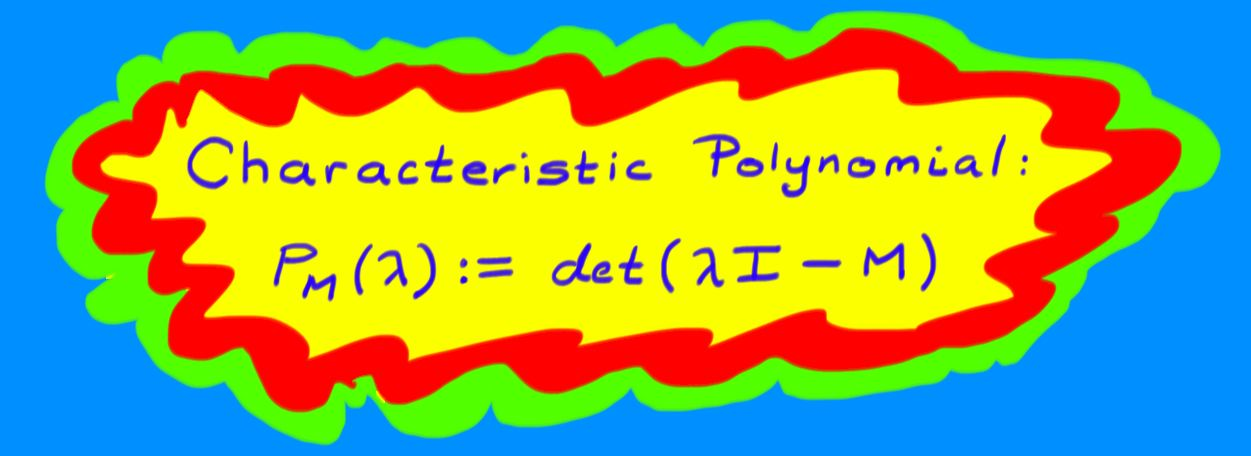
\includegraphics[scale=.3]{\eigenIIPath/charpoly.jpg}
\end{center}
\caption{Don't forget the characteristic polynomial; you will need it to compute eigenvalues.}
\end{figure}


\begin{example}
Let $L$ be the linear transformation $L \colon \Re^3\rightarrow \Re^3$ given by 
\[L\colvec{x\\y\\z}=\ccolvec{2x+y-z\\ x+2y-z\\ -x-y+2z}\, .\] 
In the standard basis the matrix $M$ representing $L$ has columns $Le_i$ for each $i$, so:

\[
\colvec{x\\y\\z} \stackrel{L}{\longmapsto} 
\begin{pmatrix}
2 & 1 & -1\\
1 & 2 & -1\\
-1 & -1 & 2\\
\end{pmatrix}\colvec{x\\y\\z}.
\]
Then the characteristic polynomial of $L$ is\footnote{It is often easier (and equivalent) to solve $\det (M-\lambda I)=0$.}
\begin{eqnarray*}
P_M(\lambda)&=&\det \begin{pmatrix}
\mc{\lambda - 2} &\mc{ -1} & \mc{1}\\
\mc{-1} &\mc{ \lambda - 2} & \mc{1}\\
\mc{1} & \mc{1} & \mc{\lambda - 2}\\
\end{pmatrix}\\[2mm]
&=& (\lambda - 2)[ (\lambda - 2)^2-1 ] + 
[-(\lambda - 2)-1 ] +
[-(\lambda - 2)-1] \\[2mm]
&=& (\lambda - 1)^2(\lambda - 4)\, .
\end{eqnarray*}
So $L$ has eigenvalues $\lambda_1=1$ (with multiplicity $2$), and $\lambda_2=4$ (with multiplicity $1$).

To find the eigenvectors associated to each eigenvalue, we solve the homogeneous system $(M-\lambda_iI)X=0$ for each $i$.

\begin{itemize}
\item[\underline{$\lambda=4$:}] We set up the augmented matrix for the linear system:
\begin{eqnarray*}
\begin{amatrix}{3}
-2 & 1 &-1 & 0 \\
1 & -2 &-1 & 0 \\
-1 & -1 &-2 & 0 \\
\end{amatrix} 
 & \sim & \begin{amatrix}{3}
1 & -2 &-1 & 0 \\
0 & -3 &-3 & 0 \\
0 & -3 &-3 & 0 \\
\end{amatrix} \\
 & \sim & \begin{amatrix}{3}
1 & 0 & 1 & 0 \\
0 & 1 & 1 & 0 \\
0 & 0 & 0 & 0 \\
\end{amatrix}. \\
\end{eqnarray*}
%So we see that $z=:t$, $y=-t$, and $x=-t$ gives a formula for eigenvectors in terms of the free parameter $t$.  
Any vector of the form $t\colvec{-1\\-1\\1}$ is then an eigenvector with eigenvalue $4$; thus~$L$ leaves a line through the origin invariant.

\item[\underline{$\lambda=1$:}]  Again we set up an augmented matrix and find the solution set:
\begin{eqnarray*}
\begin{amatrix}{3}
1 & 1 &-1 & 0 \\
1 & 1 &-1 & 0 \\
-1 & -1 & 1 & 0 \\
\end{amatrix} 
 & \sim & \begin{amatrix}{3}
1 & 1 &\!\!-1 & 0 \\
0 & 0 &0 & 0 \\
0 & 0 &0 & 0 \\
\end{amatrix}.
\end{eqnarray*}
Then the solution set has two free parameters, $s$ and $t$, such that $z=z=:t$, $y=y=:s$, and $x=-s+t$.  Thus $L$ leaves invariant the set:
\[
\left\{ s\colvec{-1\\1\\0}+t\colvec{1\\0\\1} \middle| s,t\in \Re   \right\}.
\]
This set is a plane through the origin.  So the multiplicity two eigenvalue has two independent eigenvectors, $\colvec{-1\\1\\0}$ and $\colvec{1\\0\\1}$ that determine an invariant plane.
\end{itemize}
\end{example}

\begin{example}
Let $V$ be the vector space of smooth (\textit{i.e.} infinitely differentiable) functions $f \colon \Re\rightarrow \Re$.  Then the derivative is a linear operator $\frac{d}{dx} \colon V\rightarrow V$.  What are the eigenvectors of the derivative?  In this case, we don't have a matrix to work with, so we have to make do.

A function $f$ is an eigenvector of $\frac{d}{dx}$ if there exists some number $\lambda$ such that \[\frac{d}{dx}f=\lambda f\, .\]  An obvious candidate is the exponential function, $e^{\lambda x}$; indeed, $\frac{d}{dx} e^{\lambda x} = \lambda e^{\lambda x}$.
The operator $\frac{d}{dx}$ has an eigenvector $e^{\lambda x}$ for every $\lambda \in \Re$.
%This is actually the all of the eigenvectors for $\frac{d}{dx}$. 
%(This can be proved using the fact that every infinitely differentiable function has a Taylor series with infinite radius of convergence, and then using the Taylor series to show that if two functions are eigenvectors of $\frac{d}{dx}$ with eigenvalues $\lambda$, then they are scalar multiples of each other.)
\end{example}


\section{Eigenspaces}
In the previous example, we found two eigenvectors  \[\colvec{-1\\1\\0} \mbox{ and }\colvec{1\\0\\1}\] for $L$, both with eigenvalue $1$.  Notice that  \[\colvec{-1\\1\\0} + \colvec{1\\0\\1}=
\colvec{0\\1\\1}\] is also an eigenvector of $L$ with eigenvalue $1$.  In fact, any linear combination \[r\colvec{-1\\1\\0} + s\colvec{1\\0\\1}\] of these two eigenvectors will be another eigenvector with the same eigenvalue.  

More generally, let $\{ v_1, v_2, \ldots \}$ be eigenvectors of some linear transformation $L$ with the same eigenvalue $\lambda$.  A \emph{linear combination}\index{Linear combination} of the $v_i$ is given by $c^1v_1+c^2v_2+\cdots$ for some constants $c^1, c^2,\ldots$.  Then
\begin{eqnarray*}
L(c^1v_1+c^2v_2+\cdots) &=& c^1Lv_1+c^2Lv_2+\cdots \text{ by linearity of $L$}\\
&=& c^1\lambda v_1\,+c^2\lambda v_2+\cdots \hspace{.5mm} \text{ since $Lv_i=\lambda v_i$ }\\
&=& \lambda (c^1v_1+c^2v_2+\cdots).
\end{eqnarray*}
So every linear combination of the $v_i$ is an eigenvector of $L$ with the same eigenvalue $\lambda$.
In simple terms, any sum of eigenvectors is again an eigenvector {\itshape if they share the same eigenvalue}.

The space of all vectors with eigenvalue $\lambda$ is called an {\bf eigenspace}\index{Eigenspace}.  It is, in fact, a vector space contained within the larger vector space $V$.  It contains $0_V$, since $L0_V=0_V=\lambda 0_V$, and is closed under addition and scalar multiplication by the above calculation.  All other vector space properties are inherited from the fact that $V$ itself is a vector space. In other words, the \hyperlink{sst}{subspace theorem} (\ref{subspacetheorem}, chapter~\ref{subspacesspanning}) ensures that $V_\lambda:=\{v\in V|Lv=0\}$ is a subspace of $V$.

%An eigenspace is an example of a \emph{subspace}\index{Subspace!notion of} of $V$, a notion explored in Chapter~\ref{subspacesspanning}.

\Videoscriptlink{eigenvalues_and_eigenvectors_ii_eigenspaces.mp4}{Eigenspaces}{scripts_eigenvalues_eigenvectors_ii_eigenspaces}

%\begin{center}\href{\webworkurl ReadingHomework19/1/}{Reading homework: problem \ref{evalsevectsII}.1}\end{center}
\Reading{EigenvaluesAndEigenvectors}{3}

\begin{center}
\shabox{
{\bf \hyperref[sample2]{You can now attempt the second sample midterm. 
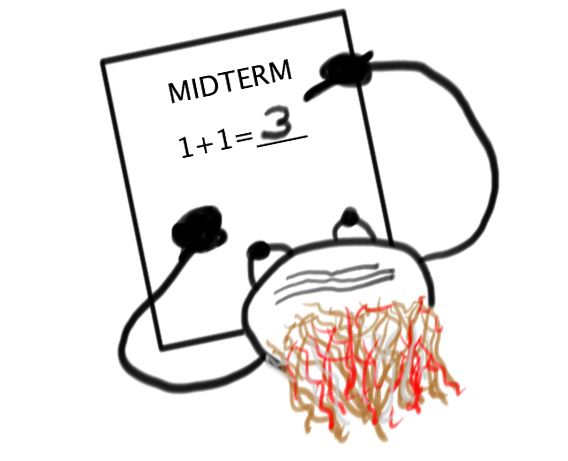
\includegraphics[scale=.15]{midterm.jpg}}}}
\end{center}
%
%\section*{References}
%Hefferon, Chapter Three, Section III.1: Representing Linear Maps with Matrices
%\\
%Hefferon, Chapter Five, Section II.3: Eigenvalues and Eigenvectors
%\\
%Beezer, Chapter E, Section EE
%\\
%Wikipedia:
%\begin{itemize}
%\item \href{http://en.wikipedia.org/wiki/Eigenvalue,_eigenvector_and_eigenspace}{Eigen*}
%\item \href{http://en.wikipedia.org/wiki/Characteristic_polynomial}{Characteristic Polynomial}
%\item \href{http://en.wikipedia.org/wiki/Linear_map}{Linear Transformations (and matrices thereof)}
%\end{itemize}


\section{Review Problems}

{\bf Webwork:} 
\begin{tabular}{|c|c|}
\hline
Reading Problems & 
 \hwrref{EigenvaluesAndEigenvectors}{1}, \hwrref{EigenvaluesAndEigenvectors}{2}, \hwrref{EigenvaluesAndEigenvectors}{3}\\
Characteristic polynomial&  \hwref{EigenvaluesAndEigenvectors}{4}, \hwref{EigenvaluesAndEigenvectors}{5}, \hwref{EigenvaluesAndEigenvectors}{6}\\
Eigenvalues &  \hwref{EigenvaluesAndEigenvectors}{7}, \hwref{EigenvaluesAndEigenvectors}{8}\\
Eigenspaces &  \hwref{EigenvaluesAndEigenvectors}{9}, \hwref{EigenvaluesAndEigenvectors}{10}\\
Eigenvectors &  \hwref{EigenvaluesAndEigenvectors}{11}, \hwref{EigenvaluesAndEigenvectors}{12},
\hwref{EigenvaluesAndEigenvectors}{13}, \hwref{EigenvaluesAndEigenvectors}{14}\\
Complex eigenvalues&\hwref{EigenvaluesAndEigenvectors}{15}\\
  \hline
\end{tabular}






\begin{enumerate}
\item \label{det33} Let $M=\begin{pmatrix}
m^1_1 & m^1_2 & m^1_3\\
m^2_1 & m^2_2 & m^2_3\\
m^3_1 & m^3_2 & m^3_3\\
\end{pmatrix}$.  Use row operations to put $M$ into \emph{row echelon form}.  For simplicity, assume that $m_1^1\neq 0 \neq m^1_1m^2_2-m^2_1m^1_2$.

Prove that $M$ is non-singular if and only if:
\[
m^1_1m^2_2m^3_3 
- m^1_1m^2_3m^3_2 
+ m^1_2m^2_3m^3_1 
- m^1_2m^2_1m^3_3 
+ m^1_3m^2_1m^3_2
- m^1_3m^2_2m^3_1
\neq 0
\]

\phantomnewpage

\item 
\begin{enumerate}
\item What does the matrix $E^1_2=\begin{pmatrix}
0 & 1 \\
1 & 0
\end{pmatrix}$ do to $M=\begin{pmatrix}
a & b \\
d & c
\end{pmatrix}$ under left multiplication?  What about right multiplication?
\item Find elementary matrices $R^1(\lambda)$ and $R^2(\lambda)$ that respectively multiply rows $1$ and $2$ of $M$ by $\lambda$ but otherwise leave $M$ the same under left multiplication.
\item Find a matrix $S^1_2(\lambda)$ that adds a multiple $\lambda$ of row $2$ to row $1$ under left multiplication.
\end{enumerate}

\phantomnewpage

\item Let $M$ be a matrix and $S^i_jM$ the same matrix with rows \(i\) and \(j\) switched.  Explain every line of the 
\hyperlink{rowswap}{series of equations} proving that $\det M = -\det (S^i_jM)$.

\phantomnewpage

%\item \label{prob_inversion_number} This problem is a ``hands-on'' look at why \hyperlink{permutation_parity}{the property} describing the parity of permutations is true.
%
%\hypertarget{inversion_number}{The \emph{inversion number}}\index{Permutation!Inversion number} of a permutation $\sigma$ is the number of pairs $i<j$ such that $\sigma(i)>\sigma(j)$; it's the number of ``numbers that appear left of smaller numbers'' in the permutation.  For example, for the permutation $\rho = [4,2,3,1]$, the inversion number is $5$. The number $4$ comes before $2,3,$ and $1$, and $2$ and $3$ both come before $1$.
%
%Given a permutation $\sigma$, we can make a new permutation $\tau_{i,j} \sigma$ by exchanging the $i$th and $j$th entries of $\sigma$.
%
%\begin{enumerate}
%\item What is the inversion number of the permutation \(\mu=[1,2,4,3]\) that exchanges 4 and 3 and leaves everything else alone? Is it an even or an odd permutation?
%
%\item What is the inversion number of the permutation \(\rho=[4,2,3,1]\) that exchanges 1 and 4 and leaves everything else alone? Is it an even or an odd permutation?
%
%\item What is the inversion number of the permutation \(\tau_{1,3} \mu\)? Compare the parity\footnote{The \emph{parity} of an integer refers to whether the integer is even or odd. Here the parity of a permutation $\mu$ refers to the parity of its inversion number.} of \(\mu\) to the parity of \(\tau_{1,3} \mu.\)
%
%\item What is the inversion number of the permutation \(\tau_{2,4} \rho\)? Compare the parity of \(\rho\) to the parity of \(\tau_{2,4} \rho.\)
%
%\item What is the inversion number of the permutation \(\tau_{3,4} \rho\)? Compare the parity of \(\rho\) to the parity of \(\tau_{3,4} \rho.\)
%\end{enumerate}
%
%\videoscriptlink{elementary_matrices_determinant_hint.mp4}{Problem~\ref{prob_inversion_number} hints}{scripts_elementary_matrices_determinants_hint}

\phantomnewpage

%\item \label{problem_permutation} (Extra credit) Here we will examine a (very) small set of the general properties about permutations and their applications. In particular, we will show that one way to compute the sign of a permutation is by finding the \hyperlink{inversion_number}{inversion number} $N$ of $\sigma$ and we have
%\[
%\sgn(\sigma) = (-1)^N.
%\]
%
%For this problem, let $\mu = [1,2,4,3]$.
%
%\begin{enumerate}
%\item Show that every permutation $\sigma$ can be sorted by only taking simple (adjacent) transpositions\index{Permutation!Simple transposition} $s_i$ where $s_i$ interchanges the numbers in position $i$ and $i+1$ of a permutation $\sigma$ (in our other notation $s_i = \tau_{i,i+1}$). For example $s_2 \mu = [1, 4, 2, 3]$, and to sort $\mu$ we have $s_3 \mu = [1, 2, 3, 4]$.
%
%\item \label{prob_part_relations} We can compose simple transpositions together to represent a permutation (note that the sequence of compositions is not unique), and these are associative, we have an identity (the trivial permutation where the list is in order or we do nothing on our list), and we have an inverse since it is clear that $s_i s_i \sigma = \sigma$. Thus permutations of $[n]$ under composition are an example of a \hyperref[groups]{group}. However note that not all simple transpositions commute with each other since
%\begin{align*}
%s_1 s_2 [1, 2, 3] & = s_1 [1, 3, 2] = [3, 1, 2]
%\\ s_2 s_1 [1, 2, 3] & = s_2 [2, 1, 3] = [2, 3, 1]
%\end{align*}
%(you will prove here when simple transpositions commute). When we consider our initial permutation to be the trivial permutation $e = [1, 2, \dotsc, n]$, we do not write it; for example $s_i \equiv s_i e$ and $\mu = s_3 \equiv s_3 e$. This is analogous to not writing 1 when multiplying. Show that $s_i s_i = e$ (in shorthand $s_i^2 = e$), $s_{i+1} s_i s_{i+1} = s_i s_{i+1} s_i$ for all $i$, and $s_i$ and $s_j$ commute for all $|i - j| \geq 2$.
%
%\item Show that every way of expressing $\sigma$ can be obtained from using the relations proved in part~\ref{prob_part_relations}. In other words, show that for any expression $w$ of simple transpositions representing the trivial permutation $e$, using the proved relations.
%
%\emph{Hint: Use induction on $n$. For the induction step, follow the path of the $(n+1)$-th strand by looking at $s_n s_{n-1} \cdots s_k s_{k\pm1} \cdots s_n$ and argue why you can write this as a subexpression for any expression of $e$. Consider using diagrams of these paths to help.}
%
%\item The simple transpositions \hyperlink{action}{acts on} an $n$-dimensional vector space $V$ by $s_i v = E^i_{i+1} v$ (where $E^i_j$ is \hyperlink{elem_matrix_row_swap}{an elementary matrix}) for all vectors $v \in V$. Therefore we can just represent a permutation $\sigma$ as the matrix $M_{\sigma}$\footnote{Often people will just use $\sigma$ for the matrix when the context is clear.}, and we have $\det(M_{s_i}) = \det(E^i_{i+1}) = -1$. Thus prove that $\det(M_{\sigma}) = (-1)^N$ where $N$ is a number of simple transpositions needed to represent $\sigma$ as a permutation. You can assume that $M_{s_i s_j} = M_{s_i} M_{s_j}$ (it is not hard to prove) and that $\det(A B) = \det(A) \det(B)$ \hyperref[detmultiplicative]{from Chapter~\ref*{elementarydeterminantsII}}.
%
%\emph{Hint: You to make sure $\det(M_{\sigma})$ is well-defined since there are infinite ways to represent $\sigma$ as simple transpositions.}
%
%\item Show that $s_{i+1} s_i s_{i+1} = \tau_{i, i+2}$, and so give one way of writing $\tau_{i, j}$ in terms of simple transpositions? Is $\tau_{i,j}$ an even or an odd permutation? What is $\det(M_{\tau_{i,j}})$? What is the inversion number of $\tau_{i,j}$?
%
%\item The minimal number of simple transpositions needed to express $\sigma$ is called the \emph{length}\index{Permutation!Length} of $\sigma$; for example the length of $\mu$ is 1 since $\mu = s_3$. Show that the length of $\sigma$ is equal to the inversion number of $\sigma$.
%
%\emph{Hint: Find an procedure which gives you a new permutation $\sigma^{\prime}$ where $\sigma = s_i \sigma^{\prime}$ for some $i$ and the inversion number for $\sigma^{\prime}$ is 1 less than the inversion number for $\sigma$.}
%
%\item Show that $(-1)^N = \sgn(\sigma) = \det(M_{\sigma})$, where $\sigma$ is a permutation with $N$ inversions. Note that this immediately implies that $\sgn(\sigma \rho) = \sgn(\sigma) \sgn(\rho)$ for any permutations $\sigma$ and $\rho$.
%\end{enumerate}

\item Let $M'$ be the matrix obtained from $M$ by swapping two columns $i$ and $j$. Show that $\det M'=-\det M $.

\item The scalar triple product of three vectors $u,v,w$ from $\Re^3$ is $u\cdot(v\times w)$. Show that this product is the same as the determinant of the matrix whose columns are $u,v,w$ (in that order). What happens to the scalar triple product when the factors are permuted? 

\item Show that if $M$ is a $3\times 3$ matrix whose third row is a sum of multiples of the other rows ($R_3=aR_2+bR_1$) then $\det M=0$. Show that the same is true if one of the columns is a sum of multiples of the others. 

\end{enumerate}

\phantomnewpage


\newpage

